%! Mode:: "TeX:UTF-8"
%! TEX program = xelatex
%\documentclass{cumcmthesis}
\documentclass[withoutpreface,bwprint]{cumcmthesis} %去掉封面与编号页,电子版提交的时候使用。
\usepackage{etoolbox}
\BeforeBeginEnvironment{tabular}{\zihao{-5}}
\usepackage{cite}
\usepackage[numbers,sort&compress]{natbib}
\usepackage[framemethod=TikZ]{mdframed}
\usepackage{url}   % 网页链接
\usepackage{subcaption} % 子标题
\title{交巡警服务平台的设置与调度}
\tihao{B}
\baominghao{4321}
\schoolname{华南理工大学}
\membera{ }
\memberb{ }
\memberc{ }
\supervisor{ }
\yearinput{2011}
\monthinput{03}
\dayinput{23}
\usepackage{yhmath}
\graphicspath{{figures/}}




\begin{document}
	
	\maketitle
	\begin{abstract}
		
		
		\keywords{\TeX{}\quad  图片\quad   表格\quad  公式}
	\end{abstract}
	
	%目录  2019 明确不要目录,我觉得这个规定太好了
	\tableofcontents
	
	\newpage
	
	\section{问题重述}
	\subsection{问题背景}
	俗话说,“有困难找警察”。警察承担着刑事执法、治安管理、交通管理、服务群众等四大职能。为了高效地发挥这些职能,在市区的交通枢纽和重要位置需要设置交巡警服务平台。每个平台的职能与警力配备基本相同,但受限于警务资源,怎样根据城市的实情以及需求合理地设置交巡警服务平台、分配管辖范围、调度警力资源是警务系统面临的一个重要课题。
	
	\subsection{问题要求}
	
	试就某市设置交巡警服务平台的相关情况,建立数学模型分析研究下面的问题:
	
	\textbf{问题1}  
	该市中心城区A的交通网络和现有的20个交巡警服务平台的设置情况如图1所示,相关的数据信息见附件2。
	
	(1)请为各交巡警服务平台分配管辖范围,以确保在其管辖范围内发生紧急事件时,交巡警能够在3分钟内到达现场(假设警车时速为60公里/小时)。
	
	(2)针对重大突发事件,需要调度全区20个交巡警服务平台的警力资源,对出入该区的13条交通要道进行快速全封锁(一个平台的警力最多封锁一个路口),请给出该区交巡警服务平台警力的合理调度方案。
	
	(3)由于目前交巡警服务平台的工作量不均衡且部分地方出警时间过长,拟在该区内再增加2至5个平台,请确定需要增加平台的具体个数和位置。
	
	\begin{figure}[H]
		\centering
		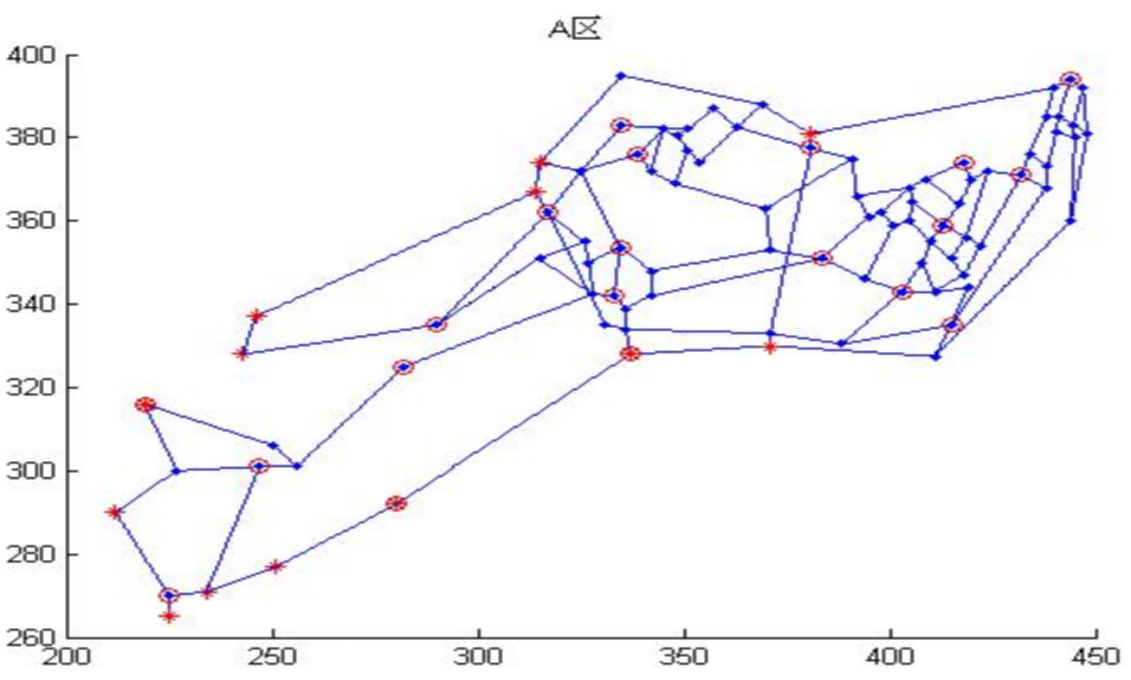
\includegraphics[width=0.6\textwidth]{A区的交通网络与平台设置的示意图.png}
		\caption{A区的交通网络与平台设置的示意图}\label{A区交通网络示意图}
	\end{figure}
	\textbf{问题2}  针对全市(主城六区A,B,C,D,E,F)的具体情况,按照设置交巡警服务平台的原则和任务,分析研究该市现有交巡警服务平台设置方案(参见附件)的合理性。如果有明显不合理,请给出解决方案。
	
	如果该市地点P(第32个节点)处发生了重大刑事案件,在案发3分钟后接到报警,犯罪嫌疑人已驾车逃跑。为了快速搜捕嫌疑犯,请给出调度全市交巡警服务平台警力资源的最佳围堵方案。
	\begin{figure}[H]
		\centering
		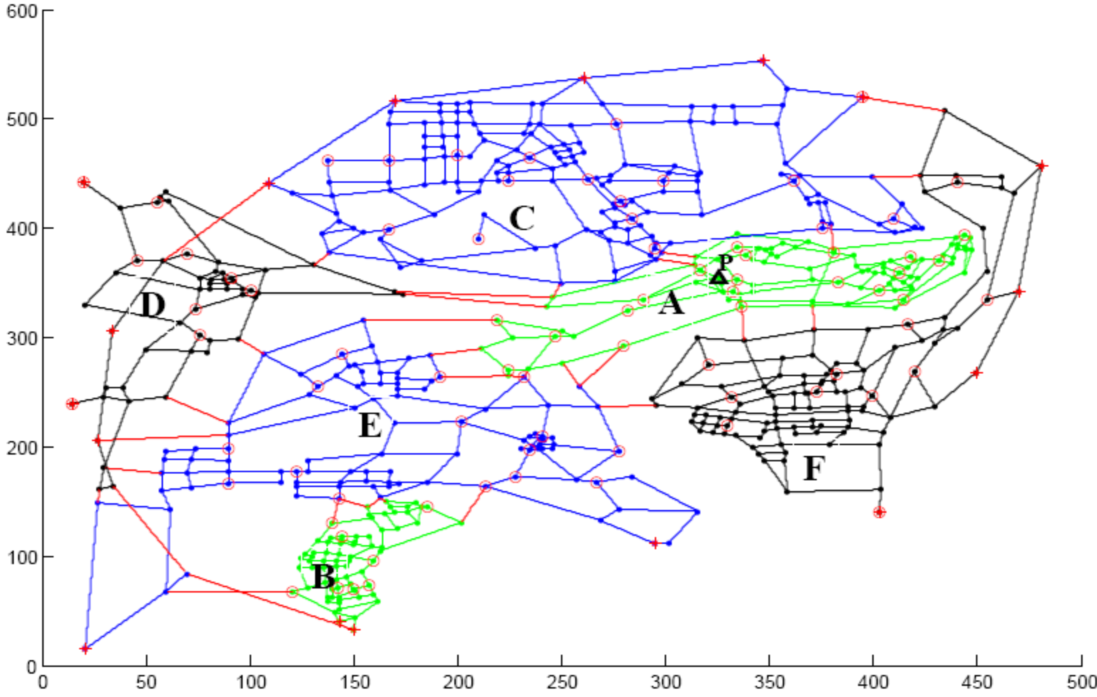
\includegraphics[width=0.6\textwidth]{全市六区交通网络与平台设置的示意图.png}
		\caption{全市六区交通网络与平台设置的示意图}\label{全市交通网络示意图}
	\end{figure}
	
	\textbf{说明:}
	\begin{enumerate}[itemindent=2em]
		\item 图中实线表示市区道路;红色线表示连接两个区之间的道路;
		\item 实圆点“·”表示交叉路口的节点,没有实圆点的交叉线为道路立体相交;
		\item 星号“*”表示出入城区的路口节点;
		\item 圆圈“○”表示现有交巡警服务平台的设置点;
		\item 圆圈加星号“○*”表示在出入城区的路口处设置了交巡警服务平台;
		\item 附图2中的不同颜色表示不同的区。 
	\end{enumerate}
	
	
	\section{问题分析}
	\subsection{问题1分析}
	第一小问:按照题目要求将92个路口分配给20个交巡警服务平台去管理,可以通过求解路口i是否受交巡警平台j管辖,进而求出最优的管辖范围分配,这是典型的0-1整数规划模型。出于朴素的思想,在理想情况下如果每个路口发生事故时都交由距离最近的交巡警平台去处理,则总时间必然为最小,由于题目中要求解出每对点之间的最短路径,所以采用了Floyd算法进行计算。
	
	第二小问:。
	
	\subsection{问题2分析}	
	第一小问:
	
	
	
	\section{模型假设}
	
	\begin{itemize}
		\item 假设在问题一中每个平台都有足够的警力可以同时管辖所属范围。
		\item 假设处理每个交通事故所需警力及时间相同。
		\item 仅考虑交通事故发生在路口的情况。
	\end{itemize}
	
	\section{符号说明}
	
	\begin{table}[H]
		\centering
		\begin{tabular}{p{2cm}<{\centering}p{9cm}<{\centering}p{2cm}<{\centering}}
			\toprule[1.5pt]
			符号 & 说明 & 单位 \\
			\midrule
			$c_i$ & 第i个路口发生事故的概率  & / \\
			$s_{i j}$ & 从路口i到交巡警平台j的最短路径 & m \\
			$v$ & 警车时速 & m/s \\
			$b$ & 警力约束 & / \\
			\bottomrule[1.5pt]
		\end{tabular}
	\end{table}
	
	\section{模型的建立和求解}
	\subsection{交巡警平台管辖范围分配}
	
	记$s_{i j}(i=1,2...,92 j=1,2...,20)$表示路口i与交巡警平台之间的距离,引进0-1变量
	\begin{center}
		$x_{i j}= \left\{ \begin{array}{ll}
			1, & \text { 将路口i分配给交巡警平台j } \\
			0, & \text { 否则 }
		\end{array}\right.$
	\end{center}
	
	目标函数为加权后的时间成本最小,即
	\begin{center}
		$\min \sum_{i=1}^{92} c_i \cdot \sum_{j=1}^{20} x_{i j} \cdot \frac{s_{i j}}{v}$
	\end{center}
	
	决策变量$x_{i j}$还应满足以下几类约束条件:
	
	首先,每一个路口都只由一个交巡警服务平台管辖,即
	\begin{center}
		$\sum_{j=1}^{20} x_{i j}=1, \text { i=1,2...,20,j=1,2...,92. }$
	\end{center}
	
	其次,每次发生事故交巡警能够在3分钟内到达现场,即
	\begin{center}
		$x_{i j} \cdot \frac{s_{i j}}{v} \leq 3×60, \text { i=1,2...,20,j=1,2...,92. }$
	\end{center}
	
	则该问题的0-1整数规划模型为
	\begin{equation}
		\min \sum_{i=1}^{92} c_i \cdot \sum_{j=1}^{20} x_{i j} \cdot \frac{s_{i j}}{v}
	\end{equation}
	\begin{equation}
		s.t. \left\{ \begin{array}{ll}
			\sum_{j=1}^{20} x_{i j}=1, & \text { i=1,2...,20,j=1,2...,92. }  \\
			x_{i j} \cdot \frac{s_{i j}}{v} \leq 3×60, & \text { i=1,2...,20,j=1,2...,92. } \\
			x_{i j} =0 \text{或1}, & \text { i=1,2...,20,j=1,2...,92. } 
		\end{array}\right.
	\end{equation}
	
	利用Matlab软件,求得最优解为\cite{Jiang2018}
	
	\begin{table}[!htbp]
		\centering
		\begin{tabular}{c c c c} %l(left)居左显示 r(right)居右显示 c居中显示
			%\hline 
			%&管辖路口\\  %横向合并7列单元格  两侧添加竖线
			
			\toprule
			交巡警平台编号 & 所管辖路口编号 & 交巡警平台编号 & 所管辖路口编号 \\
			\midrule
			1 & 78,76,75,75,73,71,69,68,67,1 & 11 & 27,,26,11,1\\
			2 & 72,7,44,43,4,3,2 & 12 & 25,12\\
			3 & 76,65,55,54 & 13 & 24,23,22,21,14,13\\
			4 & 64,63,62,6,57,4 & 14 & / \\
			5 & 59,58,56,53,52,51,5,49,5 & 15 & 29,28\\
			6 & / & 16 & 38,37,36,16\\
			7 & 61,48,47,32,3,15,7,6 & 17 & 42,41,17\\
			8 & 46,33 & 18 & 83,82,81,8,18\\
			9 & 45,35,34,31,9,8 & 19 & 79,77,19\\
			10 & / & 20 & 92,91,90,89,88,87,86,85,84,20\\
			\bottomrule
		\end{tabular}
		\caption{各个交巡警平台的路口管辖分配}
	\end{table}

	根据求解结果,作出各个交巡警平台的路口管辖分配图如下:
	\begin{figure}[htb]
		\centering
		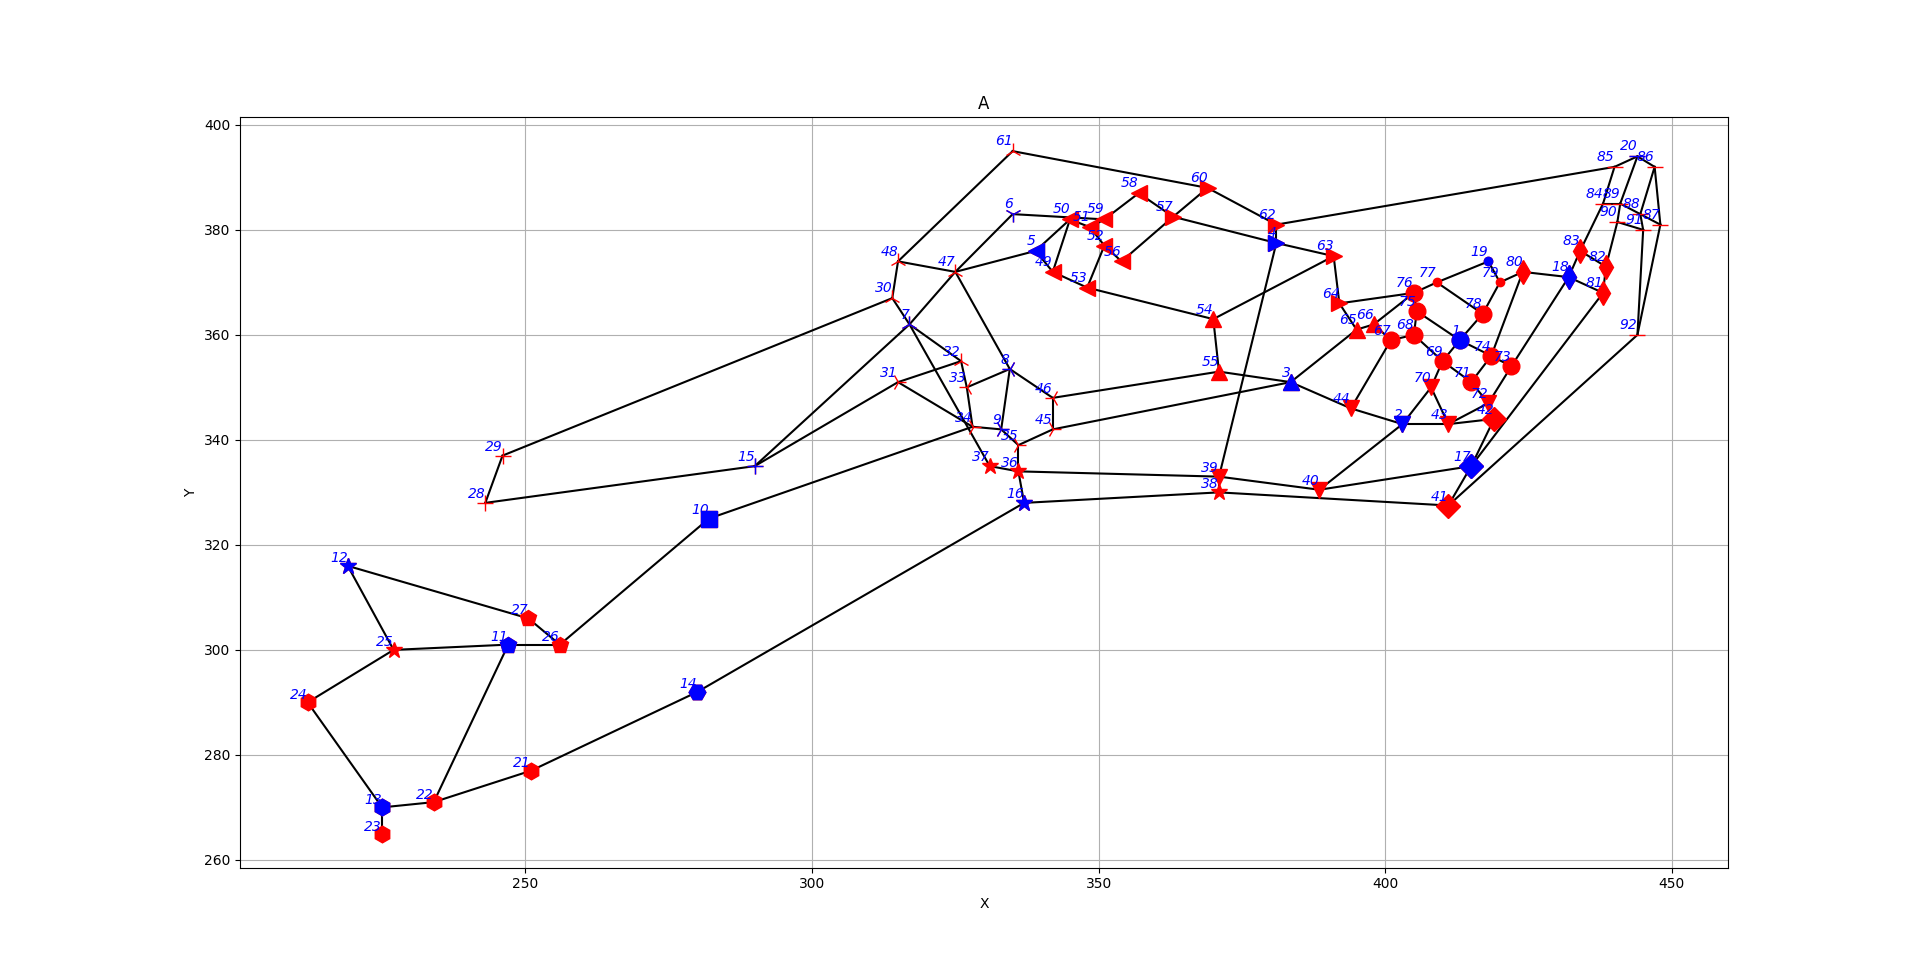
\includegraphics[width=1\linewidth]{警局管理范围图}
		\caption{各交巡警平台管辖范围分布图}
		\label{fig:各交巡警平台管辖范围分布图}
	\end{figure}

	在图\ref{fig:各交巡警平台管辖范围分布图}中,蓝色的点表示交巡警平台本身的位置,与之相同形状的路口表示由该交巡警平台进行管辖。根据题目所建立的最小值整数规划目标函数$\min \sum_{i=1}^{92} c_i \cdot \sum_{j=1}^{20} x_{i j} \cdot \frac{s_{i j}}{v}$,交巡警平台到自身的路口距离为0,必定负责自身所在路口,所以每一个交巡警平台都会负责一个或以上的点,保障了交巡警平台存在的意义。
	
	
	\section{灵敏度分析}
	
	\section{模型检验和误差分析}
	
	\section{模型的评价改进和推广}
	\subsection{模型的优点}
	\begin{itemize}
		\item 
		\item 
		\item 
		\item 
	\end{itemize}
	\subsection{模型的缺点}
	\begin{itemize}
		\item 
		\item 
		\item 
	\end{itemize}
	\subsection{模型的推广}
	
	%参考文献
	%	\begin{thebibliography}{9}%宽度9
		%		\bibitem[1]{liuhaiyang2013latex}
		%		刘海洋.
		%		\newblock \LaTeX {}入门\allowbreak[J].
		%		\newblock 电子工业出版社, 北京, 2013.
		%		\bibitem[2]{mathematical-modeling}
		%		全国大学生数学建模竞赛论文格式规范 (2020 年 8 月 25 日修改).
		%		\bibitem{3} \url{https://www.latexstudio.net}
		%	\end{thebibliography}
		\bibliographystyle{gbt7714-2005} %规定了参考文献的格式
		\bibliography{./bib/ref.bib} %调出LaTeX生成参考文献列表
	
	\newpage
	%附录
	\begin{appendices}
		\section{文件列表}
		% Table generated by Excel2LaTeX from sheet 'Sheet1'
		\begin{table}[htbp]
			\centering
			\caption{Add caption}
			\begin{tabularx}{\textwidth}{@{}c *1{>{\centering\arraybackslash}X}@{}}
				\toprule[1.5pt]
				文件名   & 文件描述 \\
				\midrule
				Data1.mat & 附件1数据 \\
				Data2.mat & 附件2数据 \\
				Data3.mat & 附件3数据 \\
				problem1.m & 问题1求解h \\
				problem2\_1.m & 问题1求解h \\
				problem2\_2.m & 问题2求解其他要求的数据 \\
				problem3.m & 问题3求解抛物面接收比 \\
				solvex0.m & 问题3球面接收比求解 \\
				linminxin.m & 灵敏性分析 \\
				huangjin.m & 黄金分割法 \\
				result.xlsx & 问题二结果表格 \\
				\bottomrule
			\end{tabularx}%
			\label{tab:addlabel}%
		\end{table}%
		\section{代码}
		%		problem1.m
		%		\lstinputlisting[language=matlab]{code/problem1.m}
		%		problem2\_1.m
		%		\lstinputlisting[language=matlab]{code/problem2_1.m}
		%		problem2\_2.m
		%		\lstinputlisting[language=matlab]{code/problem2_2.m}
		%		problem3.m
		%		\lstinputlisting[language=matlab]{code/problem3.m}
		%		solvex0.m
		%		\lstinputlisting[language=matlab]{code/solvex0.m}
		%		problem3.m
		%		\lstinputlisting[language=matlab]{code/problem3.m}
		%		linminxin.m
		%		\lstinputlisting[language=matlab]{code/linminxin.m}
		%		huangjin.m
		%		\lstinputlisting[language=matlab]{code/huangjin.m}
	\end{appendices}
	
\end{document} 